\chapter{Les grands modèles de langage~: un moyen efficace	d'automatisation de tâches archivistiques ?}

	\subsection{Les promesses des \gls{LLM}}
	
	Les promesses des \gls{LLM} sont nombreuses. Ces derniers sont entraînés 
	sur des corpus considérables de texte dans le but
	de pouvoir prédire des combinaisons de mots en réponse à une question ou
	une affirmation. Pour donner un ordre d'idée de ces quantités, Llama 3
	serait entraîné sur un corpus de plus de quinze trillions de
	\gls{token}\footcite{meta}. Un token est
	une unité de texte traitée comme une séquence distincte par le modèle, il
	peut correspondre à un mot, une partie de mot ou un symbole. Il est
	généralement admis qu'un \gls{token} est en moyenne équivalent aux trois
	quarts d'un mot. Les données d'entraînement de la base du modèle Llama 3
	contiendraient donc environ onze trillions de mots, soit environ 21 000
	milliards de fois le contenu des Misérables de Victor Hugo, ou bien 1,5
	milliard de fois le wikipédia français\footnote{Au 21 août 2024, à 16h30, le wikipédia français est composé de 2 630 307 articles
		d'une moyenne de 2 758 mots d'après cette source : \url{http://fr.wikicount.net/}}. Ces grandes quantités de données,
	provenant majoritairement du web, permettent aux modèles d'avoir des
	connaissances générales dans des domaines très divers. Ils sont
	davantage capables de générer des réponses en prenant en compte des
	contextes, qui sont alors plus pertinentes
	et cohérentes que des modèles spécialisés sur une tâche. Ils analysent
	la relation entre les mots et leur signification dans une phrase ou un
	paragraphe et le contexte de cette dernière. Par exemple, si une
	question est posée dans un contexte juridique, le modèle pourra adapter
	sa réponse en fonction de ce domaine spécifique. Par ailleurs, certains
	grands modèles de langage sont simples à utiliser grâce à des interfaces
	de discussion, on parle alors de \gls{chatbot}s ou d'\gls{générative}
	conversationnelle. C'est le cas de \emph{Chagpt}
	d'\emph{OpenAI.} En plus de cette interface, il possède une API
	(\emph{Application Programming Interface}), permettant aux développeurs
	d\textquotesingle intégrer ses capacités dans leurs applications et
	services, pour réaliser des automatisations de plus grande envergure. Il
	est également possible d'installer localement des modèles \emph{open
		source}, pour éviter de passer par des API et ainsi de transmettre des
	données. Les avantages de l'IA générative conversationnelle sont
	nombreux. Le code est beaucoup plus léger que pour l'entraînement de
	modèles maison. Il nécessite moins de compétences techniques et il est
	plus aisé de réaliser des expérimentations. Les utilisateurs peuvent
	tester ou affiner leurs \gls{prompt}s, c'est à dire les questions posées au
	\textit{LLM}, directement en ligne pour certains modèles et souvent sans
	frais. Les prix pour l'\gls{inference} via l'API des modèles payants ne sont
	pas forcément aussi élevés qu'on pourrait le croire. Au moment de la rédaction de ce mémoire,
	le prix d'un
	million de \gls{token}s (environ 750 000 mots) est de 30 \$ en entrée (c'est à
	dire dans le prompt) et 60 \$ pour un million en sortie pour
	gpt-4\footnote{Les tarifs d'OpenAI sont indiqués ici~: \url{https://openai.com/api/pricing/}}.
	
	Des réponses précises peuvent être générées par ces modèles en un ou
	plusieurs prompts et il est possible de les guider pour les améliorer. 
	C'est le concept du \emph{few-shots learning~}:
	l'utilisateur fournit des exemples de la tâche à remplir par le modèle
	dans son prompt pour guider ce dernier. Ces possibilités évitent d'avoir
	à développer des modèles maison spécialisés. Si les réponses ne sont pas
	assez précises, on peut aussi \emph{fine-tuner}, c'est à dire affiner
	les modèles sur des tâches spécifiques en les entraînant sur un corpus
	de prompts et de réponses à ces derniers mais cela demande beaucoup de
	temps et de capacités matérielles\footcite{wei_finetuned_2022}.
	De nouvelles recherches sont constamment menées sur les manières
	d'améliorer les réponses générées. Une discipline, le \emph{prompt
		engineering}, a émergé~: il s'agit de l'optimisation des prompts afin
	d'obtenir les meilleures réponses possibles, via l'ajout d'exemples dans
	le \textit{prompt}, la contextualisation et beaucoup d'autres techniques. Les
	modèles évoluent aussi rapidement que la recherche avance donc il faut
	constamment être à jour sur les dernières publications et recherches
	menées, d\textquotesingle où la présence de nombreuses références à des
	\emph{preprints} dans ce mémoire. Les plus grands modèles ont par ailleurs 
	l'avantage de gérer le multilinguisme et peuvent réaliser des tâches de
	traduction. 5~\% des données d'entraînement de Llama 3 sont «~des
	données de haute qualité non anglophones couvrant plus de trente
	langues\footcite{meta}~» {[}traduction libre{]}. Des modèles
	multimodaux capables de traiter du texte et de l'image, voire du son et
	de la vidéo font en outre leur apparition.\newline
	
	Les possibilités d'usage de ces modèles semblent infinies. En ce
	qui concerne le traitement des archives, un article de chercheurs de l'université de Wuhan et de Loughborough liste des
	perspectives d'usage\footcite{zhang_archives_2024},
	que nous résumerons en plusieurs catégories~:
	
	\begin{itemize}
		\item
		Contenu des documents~: océrisation, correction d'océrisation
		\item
		Description~: repérage et génération de métadonnées (titres, dates),
		indexation, résumé
		\item
		Communication~: repérage de données sensibles, détermination de durées
		de rétention, gestion des accès utilisateurs
		\item
		Médiation~: réponses aux questions des chercheurs sur les archives et
		le domaine de l'archivistique, aide à la recherche, recommandations
		\item
		Reporting~: statistiques sur les documents conservés, sur les
		interactions avec les usagers, prédictions sur les documents qui
		seront consultés
	\end{itemize}
	
	Les \gls{LLM} peuvent donc être utilisés à différentes étapes du traitement
	des archives.
		Les perspectives sont séduisantes, mais qu'en est-il de la pratique~?
	 Les \emph{LLM} sont des bons
	outils pour les tâches simples liées au langage mais ne le sont pas pour
	les tâches complexes de raisonnement\footcite{noauthor_medium_nodate}.
	Les \emph{LLM} fonctionnent effectivement en se basant sur
	des raisonnements  mathématiques pour prédire les combinaisons de mots les plus
	probables en réponse à une entrée donnée. Leur «~intelligence~»
	apparente résulte d\textquotesingle une analyse mathématique de vastes
	ensembles de données textuelles, sans processus de compréhension ou
	réflexion. Cela
	limite leur efficacité sur des tâches nécessitant un raisonnement
	complexe. Les \emph{LLM} sont donc avant tout des outils puissants pour générer
	du texte, mais ils restent au fond des systèmes de prédiction. Face à
	des modèles généraux qui seraient incapables de véritablement raisonner,
	et donc dépourvus de l'intelligence artificielle qui leur est attribuée,
	quelles contributions concrètes les \emph{LLM} peuvent-ils réellement offrir
	dans le domaine des archives ? Quelles sont les perspectives concrètes
	d'automatisation~?
	

\subsection{La réalité archivistique~: les possibilités d'automatisation dans les processus métier}
	
	Il convient ici d'étudier les réelles possibilités d'automatisation de
	processus métier grâce aux \emph{LLM}, en commençant par présenter leurs
	apports dans le cadre du projet InventAIre. Pour ce projet, après des
	tests sur plusieurs modèles, présentés dans la note méthodologique en
	annexe, notre choix s'est porté sur l'usage du \emph{LLM} \emph{Llama 3 7B} de
	\emph{meta}, quantisé\footnote{cf. \gls{quantization} dans le glossaire.}, c'est-à-dire avec une précision réduite. Nous ne
	l'avons pas \emph{fine-tuné}. Nous posions un \textit{\gls{prompt}} par colonne à
	remplir dans l'inventaire en fournissant du contexte et le texte d'un
	document ou d'une partie de document en entrée. Un exemple de prompt
	se trouve dans le chapitre 10.
	
	Les statistiques de précision réalisées sur l'inventaire d'une
	arborescence de 420 répertoires et documents sont les suivantes~:
	
\begin{longtable}{|>{\centering\arraybackslash}p{0.22\textwidth}|>{\centering\arraybackslash}p{0.22\textwidth}|>{\centering\arraybackslash}p{0.22\textwidth}|>{\centering\arraybackslash}p{0.22\textwidth}|}
	\hline
	\textbf{Qualité de la réponse} & \textbf{Ensemble des colonnes} & \textbf{Titre et description} & \textbf{Données sensibles} \\
	\hline
	\endhead
	Correcte & 77\% & 71\% & 79\% \\
	\hline
	Incomplète/sujette à débat & 10\% & 22\% & 6\% \\
	\hline
	Incorrecte & 13\% & 6\% & 15\% \\
	\hline
\end{longtable}


	
	Beaucoup de titres et descriptions sont incomplets ou sujets à
	débat (22\%), mais il s'agit des colonnes comportant le moins de réponses
	totalement incorrectes. L'usage de ce modèle s'est donc révélé
	particulièrement pertinent sur la génération de titres et de
	descriptions. Il s'agit d'une tâche de traitement de langage qui ne
	demande pas de capacités de raisonnement et sur laquelle les
	performances des \emph{LLM} sont bonnes. Ces titres et descriptions peuvent
	permettre de faciliter la recherche dans les archives et d'interpréter
	des documents ou unités de description dont le nommage
	serait obscur. Il s'agit là de l'automatisation d'une base du travail
	de l'archiviste. Cela permet de gagner beaucoup de temps. La rédaction
	des descriptions peut en effet être longue. Pour que cette description
	soit optimale, un \gls{fine-tuning} est envisageable. Nous avons
	précédemment abordé le projet LlaMandement de la Direction générale des Finances publiques. Le \textit{fine-tuning} de
	Llama 2 a permis de produire des résumés davantage neutres. Les
	performances sont décrites comme satisfaisantes sur le point
	éthique\footcite{gesnouin_llamandement_2024}. Le système développé réduit
	significativement la charge de travail des agents, qui n'ont que des tâches de
	vérification à faire.\newline
	
	Dans les \textit{prompts} de génération des titres et descriptions, nous
	demandions au modèle d'intégrer les mots importants pour l'indexation
	des documents ou dossiers. L'objectif était d'obtenir
	de meilleurs résultats en cas de recherche plein texte sur une
	personne, une organisation, un mot matière ou un événement. Cette
	approche a produit de meilleures descriptions avec une valeur ajoutée
	pour la recherche. Les \emph{LLM} sont performants sur l'indexation automatique
	grâce à leur capacité à traiter le langage. Un projet récemment mené en
	collaboration entre l'université de Stanford et l'université de North
	Texas avait pour but d'étudier le potentiel de \emph{ChatGPT} sur la
	génération de métadonnées\footcite{noauthor_comparative_nodate}.
	L\textquotesingle étude, basée sur un échantillon de cent rapports
	gouvernementaux, a révélé que \emph{ChatGPT} est capable de produire des
	métadonnées avec une précision variable, affichant des résultats
	prometteurs pour des attributs tels que les titres et les descriptions,
	mais rencontrant des difficultés avec des normes spécifiques tels que
	les \emph{Library of Congress Subject Headings (LCSH)} et les
	\emph{Library of Congress Name Authority Files (LCNAF)}. \emph{ChatGPT}
	n\textquotesingle est pas encore pleinement performant et ne remplace
	pas les catalogueurs et catalogueuses. Le grand modèle de langage reste cependant une aide qui permet
	d'accélérer le travail de ces derniers. 
	
	Un autre projet de catalogage par
	LLM a été mené dans le but d'automatiser la génération de
	\emph{LCSH}, notices normées d'indexation matière,
	sur des thèses et des articles\footcite{chow_experiment_2024}.
	Les conclusions sont les mêmes~: \emph{ChatGPT} fait gagner du temps mais ne
	remplace pas les catalogueurs qui doivent vérifier ce qui a été généré
	et apporter des améliorations. L'article présentant les résultats du
	projet mentionne la possibilité que des données telles que des notices
	MARC et des \emph{LCSH} soient présentes dans les données d'entraînement de
	\emph{ChatGPT}. 	
	Envisager l\textquotesingle automatisation de la
	description des fonds en XML EAD pourrait ainsi être une voie prometteuse. En
	posant des questions à Llama 3 et ChatGPT sur le format nous avons
	constaté qu'ils avaient une certaine familiarité avec ce dernier, ce qui
	suggère la présence d'instruments de recherche EAD dans leurs données
	d'entraînement. En fournissant aux modèles de langage de la
	documentation bien structurée sur la norme à suivre, par exemple le
	dictionnaire des balises de l'XML EAD et/ou des exemples d'instruments
	de recherche, avec le texte d'un document ou groupe de documents, une
	potentielle automatisation de la description archivistique semble
	envisageable. Les archivistes pourraient alors se concentrer sur la
	correction et l'amélioration des résultats, ce qui permettrait de gagner
	du temps. Cependant, il est important de noter que les capacités de
	traitement des \emph{LLM} sont limitées par leur {fenêtre} de contexte, c'est à
	dire la quantité maximale de texte qu'ils peuvent analyser en une fois.\newline
	
	En ce qui concerne le repérage des données sensibles, qui représentent
	neuf colonnes dans notre inventaire et qui est primordial afin d'assurer
	la communicabilité des archives, nos tentatives avec Llama 3 révèlent un
	certain manque de précision, avec 15~\% d'erreurs dans notre évaluation.
	Des colonnes sont plus aisées à remplir que d'autres~: la colonne
	pour laquelle la précision est la meilleure est celle sur la
	«~Prévention, recherche ou poursuite de faits punissables~» avec 93\% de
	bonnes réponses, 5\% de réponses sujettes à débat et 2\% de réponses
	incorrectes. Les données personnelles et les informations sur des
	«~affaires portées devant les instances juridictionnelles,
	extrajudiciaires, disciplinaires~» étaient quant à elles plus difficiles
	à repérer. Cela est lié à la subjectivité de la définition, au fait que
	nous ayons utilisé une version réduite du modèle et au fait que le
	repérage de ces données demande une certaine capacité d'analyse. 
	
	Nous
	n'avons pas trouvé mention d'autres projets basés sur des \emph{LLM} ayant
	abouti à la détection de données sensibles. Nous avons seulement
	trouvé mention de projets d'anonymisation. Nous citerons ici deux
	articles. Le premier, «~Large Language Models are Advanced Anonymizers~»
	évoque le fait que les \emph{LLM} ont pour avantage de générer une
	anonymisation qui laisse le texte compréhensible\footcite{anony}. L'anonymisation est en effet une tâche complexe. Cette
	complexité est illustrée dans le second article, «~Robust
	Utility-Preserving Text Anonymization Based on Large Language Models~»
	par l'exemple d'un «~joueur de tennis~», «~tennis athlete~», à anonymiser
	en «~athlete~», que l'on remplacerait sûrement par «~sportif~» en
	français\footcite{yang_robust_2024}. D'après les auteurs, le modèle développé dans le
	cadre de leur étude surpasserait les modèles existants en matière
	d'anonymisation\footcite{yang_robust_2024}. Le modèle développé est un
	affinage d'un \emph{LLM} grâce à la méthode de la \emph{DPO (Direct Preference
		Optimization)}\footnote{Pour plus d'informations sur la DPO :
		\url{https://arxiv.org/pdf/2305.18290}}. Si le modèle est performant sur la
	tâche d'anonymisation, il n'est pas impensable qu'il le soit sur la
	détection de données personnelles, puisque ces dernières sont modifiées
	par le processus d'anonymisation.
	
	Les \emph{LLM} performent donc bien sur des tâches de description et
	d'indexation, surpassant les approches traditionnelles de \gls{TAL} lorsqu'elles ne sont pas approfondies et affinées sur des corpus spécifiques. Cependant, la question
	de l\textquotesingle ampleur exacte de ces performances est
	difficilement analysable. Elle nécessiterait des recherches plus
	poussées afin d'en évaluer pleinement la portée.
	L\textquotesingle intégration des différentes tâches archivistiques,
	telles que la description, l\textquotesingle indexation, et
	potentiellement d\textquotesingle autres fonctions, dans un outil basé
	sur un seul \emph{LLM} représente une perspective prometteuse. Un outil
	tout-en-un permettrait de réaliser des économies en ressources et en
	processus. C'est ce qu'ont tenté de réaliser des chercheurs de
	l'université de Wuhan et de Loughborough avec \emph{ArcGPT}, un modèle
	de sept milliards de paramètres spécifiquement développé pour réaliser des
	tâches archivistiques\footcite{zhang_arcgpt_2023}.
	Le développement ou le \gls{fine-tuning} d'un \emph{LLM} sur des tâches archivistiques
	précises pourrait ainsi permettre d'alléger les modèles tout en les rendant
	plus précis et utiles pour les archivistes.
	
	Par ailleurs, une dernière perspective permettant des économies de
	moyens est l'annotation par les \emph{LLM} pour générer les données d'entraînement de
	modèles plus légers, basés par exemple sur les méthodes traditionnelles
	du \gls{TAL}. Un article intitulé «~Large Language Models as Annotators:
	Enhancing Generalization of NLP Models at Minimal Cost~» illustre cette
	approche. Il aborde les difficultés de généralisation des modèles de
	\gls{TAL} et le besoin constant de fournir de nouvelles données
	d\textquotesingle entraînement\footcite{llm_ann}. Il propose
	l\textquotesingle annotation automatisée par des \emph{LLM} pour améliorer la
	généralisation, notamment dans les domaines où les données sont rares.
	Le principal défi réside dans le choix de données appropriées pour
	renforcer le modèle sans nuire à sa précision. Avec une automatisation
	des annotations, des économies peuvent être réalisées sur les coûts en
	personnel et sur les moyens matériels par le
	développement des modèles légers, plus aisés à déployer sans
	intermédiaire.
	\linebreak
	
	Pour conclure cette section, les possibilités
	d\textquotesingle automatisation des processus métier dans le domaine
	des archives grâce aux \emph{LLM} sont vastes. Néanmoins, les applications
	concrètes restent limitées, notamment en raison des difficultés liées à
	leur intégration dans les processus existants et à des incertitudes quant
	à la précision des résultats produits. L'IA ne peut pas remplacer l'archiviste mais
	elle pourrait accélérer son travail. Le secteur archivistique luxembourgeois
	n\textquotesingle est pas encore mature en matière de déploiement de ces
	technologies et un travail de recherche et de développement important
	reste à accomplir. Les \emph{LLM} étant des technologies récentes, des
	recherches et des tests devraient continuer afin d'explorer leurs
	apports, mais le recul sur ces dernières est pour l'instant limité.
	

	\subsection{Au delà des usages métier~: RAG, recherche et médiation}
	
	De la même manière que pour le traitement automatique du langage et des
	images détaillés dans le chapitre précédent, les usages les plus simples
	à mettre en production sont ceux qui ont les impacts les moins
	importants en cas d'erreur en termes de sécurité et de transparence.
	Plusieurs services d'archives et bibliothèques mettent à profit les \emph{LLM}
	pour des tâches de médiation avec leurs usagers. Ces projets ont
	l'avantage de demander moins de temps et de budget que ceux à
	grand impact.
	
	Une des contraintes des \emph{LLM} réside dans la limitation de leurs données
	d'entraînement. Elles sont certes volumineuses, mais ne
	permettent pas de répondre à toutes les questions. Ce sont des modèles
	faits pour générer du langage et non des réponses factuelles.
	 Une solution a été développée face à ce problème.
	Il s'agit du \gls{RAG}, technique permettant
	de récupérer des informations pertinentes au sein d'une base de connaissance pour répondre au \textit{\gls{prompt}} d'un
	utilisateur. Cette récupération se
	fait par mesure de similarité entre un document et le prompt. Les
	documents et le prompt peuvent être vectorisés avec des algorithmes tels
	que TF/IDF pour les versions légères, mais pour avoir un résultat le
	plus précis possible, ce sont souvent les \gls{embeddings} de grands modèles de
	langage\footnote{Ces méthodes ont été détaillées dans le chapitre 4.} qui
	sont utilisés. Le ou les passages pertinents pour
	répondre au \textit{prompt}, donc les plus proches de ce dernier dans l'espace
	vectoriel, sont ajoutés à la \gls{fenêtre} de lecture du \emph{LLM}, qui peut se
	baser dessus afin de générer sa réponse et peut être en mesure de citer
	ses sources\footcite{lewis_retrieval-augmented_2020}.
	
	L'application principale du \gls{RAG} dans le domaine des archives est la
	recherche d'informations ou de documents en langage naturel. En
	intégrant une base de connaissance contenant des fonds numérisés ou
	nativement numériques, l'usager peut poser des questions en langage
	naturel sur les fonds, ou éventuellement sur le fonctionnement du
	service. On peut s'interroger sur l'efficacité de cette méthode pour le
	chercheur par rapport à un moteur de recherche classique. Un moteur de
	recherche classique offre davantage de réponses en moins de temps, plus
	rapidement analysables par le chercheur, qui peut aussi jouer avec des
	filtres. Il doit néanmoins aller lire chaque document, ce qui peut lui
	faire perdre du temps. Le \emph{RAG} peut donc paraître plus efficace qu'un moteur de
	recherche pour la recherche d'une seule information précise, mais ne l'est pas
	forcément pour la recherche de documents.\newline
	
	Au Luxembourg, quelques outils basés sur le \emph{RAG} ont récemment été mis à
	disposition du grand public. A la BNL, une version beta d'un
	\gls{chatbot} a été mise en ligne fin 2023. Ce \emph{chatbot} offre la
	possibilité de poser des questions sur l'histoire luxembourgeoise en se
	basant sur des articles de presse anciens\footcite{noauthor_eluxemburgensialu_2023}.
	L'interface est similaire à celle de ChatGPT, avec une zone pour écrire
	un message, un historique conversationnel et des réponses en langage
	naturel. L'architecture technique est aussi basée sur le modèle GPT.
	La seule différence est la section «~Ma réponse se base sur les articles
	suivants~», où sont citées les sources. Le \textit{chatbot} est décrit comme un «~service
	complémentaire et expérimental\footcite{noauthor_eluxemburgensia_nodate}~»
	à la barre de recherche. Il sert à obtenir des réponses rapides et
	sourcées sur des faits historiques au Luxembourg et identifier des documents qui
	en parlent. C'est assez efficace pour une recherche rapide, mais un
	chercheur devra sans doute aller plus loin, ce qui est toutefois une composante naturelle de son travail. Il s'agit
	d'un bon outil de médiation pour le grand public, qui impressionne par
	ailleurs. Dans ce domaine, le Parlement européen a lancé \emph{Archibot 3.0},
	agent conversationnel auquel il est possible de poser des questions sur
	l'histoire législative européenne et dont la base de
	connaissance est composée d'archives numérisées de l'institution. 

	
	\begin{figure}
		\centerline{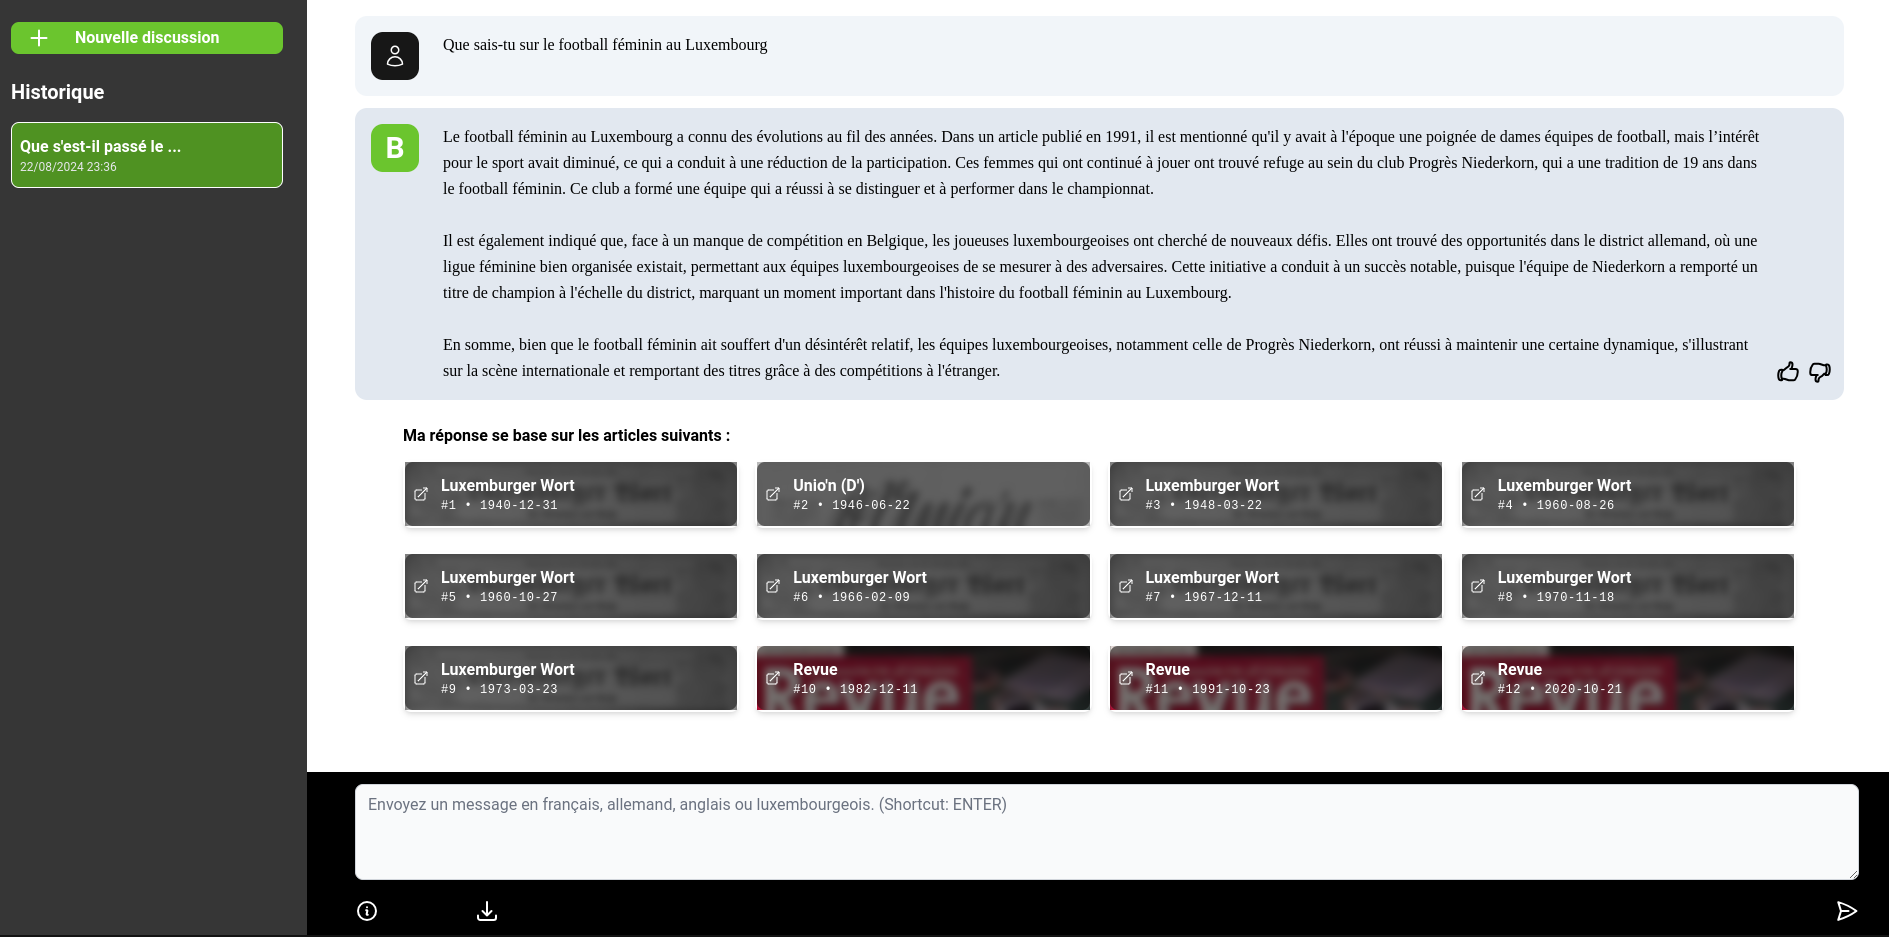
\includegraphics[width=\textwidth]{./media/image5.png}}
		\caption{Capture d'écran de l'interface du chatbot de la BNL \emph{eLuxemburgensia} }
	\end{figure}

		
		Le \emph{RAG} est une perspective intéressante en ce qui concerne la médiation dans le domaine des
	archives. Ce type d'agents joue
	un rôle dans le développement d'une forme de transparence des
	administrations avec le public mais ne remplace pour l'instant pas la
	description et l'indexation dans un moteur de recherche. Néanmoins, ces
	initiatives contribuent à procurer une visibilité plus accrue aux
	services d\textquotesingle archives, les éloignant de
	l\textquotesingle image stéréotypée de lieux poussiéreux, sombres et peu
	accessibles. Elles les présentent comme des lieux modernes et innovants.
	Elles montrent que les archives sont ouvertes à tous et à toutes, y compris au grand
	public, et pas seulement aux chercheurs ou aux passionnés de généalogie.
	Cette amélioration de l\textquotesingle image des services et cette
	démarche de médiation peuvent servir à mieux faire saisir
	l\textquotesingle importance des archives, tant au public qu'aux
	administrations dans leur ensemble et à encourager les
	investissements.\newline
	
	Les usages des grands modèles de langage et en particulier de
	l'intelligence générative conversationnelle sont donc divers dans les
	archives. Il est plus aisé de mettre en place ces technologies
	lorsqu'elles ont un faible impact en cas d'erreur. Il y a pour l'instant
	peu de recul sur ces dernières. Les \emph{LLM} ont l'inconvénient d'être
	très généraux, nécessitant d'ajuster les prompt avec des informations
	précises, des sources ou de les affiner sur des données spécifiques au
	domaine archivistique. Leur implémentation demande des connaissances
	techniques et des investissements matériels. Les recherches à venir les
	rendront peut-être plus performants sur des tâches archivistiques
	complexes ou plus légers. L'IA a un grand potentiel dans les archives
	mais nous en sommes encore au début de ses applications dans le domaine.
	Même si les projets ne conduisent pas encore à l'automatisation de
	processus complexes, ils peuvent avoir des apports connexes divers.
	
